\chapter{Literature Review}\label{sec:literature-review}

\section{Classical Relay Strategies}\label{sec:classical-relay-strategies}

The fundamental question that motivates this thesis is: can a learned relay function \(f_\theta(\cdot)\) outperform the classical relay functions (AF scaling, DF regeneration) by exploiting patterns in the received signal that analytical methods do not capture? This question is particularly relevant at low SNR, where both AF (noise amplification) and DF (decoding errors) have well-known limitations, and where the non-linear decision boundary learned by a neural network may provide a substantive advantage.

\subsection{Amplify-and-Forward (AF).}\label{sec:classical-relay-strategies-af} 
The AF relay amplifies the received signal by a gain factor \(G\) that normalizes the output power: (Equation~\ref{eq:af-gain})
\addcontentsline{equ}{listequations}{\protect\numberline{\theequation}\quad af-gain}


\begin{equation}\protect\phantomsection\label{eq:af-gain}{G = \sqrt{\frac{P_{\text{target}}}{\mathbb{E}[|y_R|^2]}}
}\end{equation} 

The end-to-end SNR for AF relay is: (Equation~\ref{eq:af-snr})

\begin{equation}\protect\phantomsection\label{eq:af-snr}{\text{SNR}_{\text{eff}}^{\text{AF}} = \frac{\text{SNR}_1 \cdot \text{SNR}_2}{\text{SNR}_1 + \text{SNR}_2 + 1}
}\end{equation} 
\addcontentsline{equ}{listequations}{\protect\numberline{\theequation}\quad af-snr}

This expression reveals a fundamental limitation: even when one hop has high SNR, the effective SNR is bottlenecked by the weaker hop. Moreover, the relay amplifies both signal and noise from the first hop, leading to noise accumulation at the destination.

\subsection{Decode-and-Forward (DF)}\label{sec:classical-relay-strategies-df} 
The DF relay demodulates the received signal, recovers the transmitted bits, and re-modulates clean symbols:

\begin{equation}\protect\phantomsection\label{eq:df-demod-remod}{\hat{b}_R = \text{demod}(y_R), \quad x_R = \text{mod}(\hat{b}_R)
}\end{equation} 
\addcontentsline{equ}{listequations}{\protect\numberline{\theequation}\quad df-demod-remod}

The end-to-end BER for DF is: (Equation~\ref{eq:df-ber-hops})

\begin{equation}\protect\phantomsection\label{eq:df-ber-hops}{P_e^{\text{DF}} = P_{e,1} + (1 - P_{e,1}) \cdot P_{e,2}
}\end{equation} 
\addcontentsline{equ}{listequations}{\protect\numberline{\theequation}\quad df-ber-hops}

where \(P_{e,1}\) and \(P_{e,2}\) are the BER of the first and second hops, respectively. For BPSK modulation over AWGN (real-valued noise with variance \(1/\text{SNR}\)), each hop's BER is \(P_e = Q\left(\sqrt{\text{SNR}}\right)\). DF provides clean regeneration at high SNR but suffers from error propagation when the first-hop BER is non-negligible.

\subsection{Other Classical Relay Techniques}

AF and DF represent two canonical extremes of the relay processing spectrum: AF performs minimal processing (linear scaling) while DF performs maximal classical processing (full regeneration). Additional techniques (e.g. CF, EF, CoF) occupy intermediate points along this spectrum. In this thesis, the AI-based relay strategies are designed to \emph{learn} the optimal relay processing function from data, potentially discovering strategies that subsume or outperform these fixed classical schemes. The focus on AF and DF as classical baselines is therefore deliberate: they bracket the classical design space and provide clear lower and upper bounds against which the learned strategies can be evaluated. These additional relay strategies are reviewed for completeness; they are not simulated in this thesis because the studied system assumes a two-hop link without a direct source-destination path.

\section{Machine Learning in Wireless Communication}\label{sec:machine-learning-in-wireless-communication}

The application of machine learning to physical-layer wireless communication has gained significant momentum in recent years, driven by the ability of neural networks to learn complex non-linear mappings directly from data. Deep learning has been applied to channel estimation \cite{YeLiJuang2018OFDMDL}, signal detection \cite{SamuelDiskinWunder2019MIMODetect}, autoencoder-based end-to-end communication \cite{Dorner2018OverTheAirDL}, and resource allocation \cite{Sun2018LearnToOptimize}. These approaches learn complex mappings from data, potentially outperforming hand-crafted algorithms in scenarios where analytical solutions are intractable or suboptimal.

\subsection{Theoretical Basis: Universal Approximation and Denoising}\label{sec:theoretical-basis-universal-approximation-and-denoising}

The theoretical justification for applying neural networks to relay signal processing rests on two pillars. First, the \textbf{universal approximation theorem} \cite{GoodfellowBengioCourville2016DeepLearning} guarantees that a feedforward network with a single hidden layer and a non-linear activation function can approximate any continuous function on a compact domain to arbitrary accuracy, given sufficient width. For relay denoising, the target function maps noisy observations to clean transmitted symbols:

\begin{equation}\protect\phantomsection\label{eq:optimal-denoiser}{f^*: \mathbb{R}^{2w+1} \to [-1, 1], \quad f^*(y_{i-w}, \dots, y_{i+w}) = \mathbb{E}[x_i \mid y_{i-w}, \dots, y_{i+w}]
}\end{equation} 
\addcontentsline{equ}{listequations}{\protect\numberline{\theequation}\quad optimal-denoiser}


This conditional expectation \(f^*\) is the Bayes-optimal denoiser : it minimizes the mean squared error (MSE) over all possible estimators. For BPSK symbols corrupted by AWGN, \(f^*\) reduces to the posterior mean:

\begin{equation}\protect\phantomsection\label{eq:optimal-denoiser-awgn}{f^*(y) = \tanh\left(\frac{y}{\sigma^2}\right)
}\end{equation} 
\addcontentsline{equ}{listequations}{\protect\numberline{\theequation}\quad optimal-denoiser-awgn}

which is a smooth sigmoid-like function that approaches the hard-decision signum function as \(\sigma^2 \to 0\) (high SNR). A neural network with a single hidden layer and tanh output can represent this function exactly, explaining why even a 169-parameter network suffices for this task.

Second, the \textbf{bias-variance decomposition} provides a framework for understanding model complexity:

\begin{equation}\protect\phantomsection\label{eq:bias-variance-decomp}{\mathbb{E}[(\hat{x} - x)^2] = \text{Bias}^2(\hat{x}) + \text{Var}(\hat{x}) + \sigma^2_{\text{irreducible}}
}\end{equation} 
\addcontentsline{equ}{listequations}{\protect\numberline{\theequation}\quad bias-variance-decomp}

The irreducible noise \(\sigma^2_{\text{irreducible}}\) represents the minimum achievable MSE, determined by the channel noise. Increasing model complexity (more parameters) reduces bias but increases variance. For the relay denoising task, the target function \(f^*\) is simple (essentially a soft threshold), so the bias term is already small for modest networks. Adding parameters beyond this point primarily increases variance (overfitting), explaining the inverted-U relationship between model size and BER observed in this thesis.

\subsection{Prior Work in Deep Learning for Physical-Layer Processing}\label{sec:prior-work-in-deep-learning-for-physical-layer-processing}

Ye et al.~\cite{YeLiJuang2018OFDMDL} demonstrated that deep neural networks can jointly perform channel estimation and signal detection in OFDM systems, achieving near-optimal performance with lower complexity than separate estimation and detection stages. Their key insight was that the DNN implicitly learns the channel's statistical structure, eliminating the need for explicit pilot-based estimation.

Samuel et al.~\cite{SamuelDiskinWunder2019MIMODetect} proposed DetNet, an unfolded projected gradient descent network for MIMO detection. By unrolling iterative optimization into a fixed number of neural network layers, DetNet achieves near-maximum-likelihood detection performance with \(O(N_t^2)\) complexity instead of the exponential complexity of exhaustive ML search. This demonstrates the power of incorporating domain knowledge (the iterative structure of the detection problem) into the network architecture.

Dorner et al.~\cite{Dorner2018OverTheAirDL} proposed treating the entire communication system : modulator, channel, and demodulator : as an autoencoder, trained end-to-end to minimize bit error rate. This approach jointly optimizes all components, potentially discovering novel modulation and coding schemes that outperform separately designed modules. The autoencoder paradigm is conceptually related to the relay processing task: (Equation~\ref{eq:mamba-selective}) both involve learning an encoder-decoder pair that maps through a noisy channel.

Sun et al.~\cite{Sun2018LearnToOptimize} applied deep learning to the NP-hard problem of resource allocation in interference networks, demonstrating that a DNN can learn near-optimal power control policies orders of magnitude faster than conventional iterative algorithms.

In the context of relay-assisted communication systems, most existing works employ neural networks primarily for \emph{relay-selection} and \emph{resource-allocation}, particularly in decode-and-forward (DF) relaying scenarios, where learning-based classifiers or predictors are used to identify the optimal relay based on channel state information, signal-to-noise ratios, or energy constraints, while the underlying relay operation remains conventional \cite{Akdemir2024DLRelaySelection}. 

A broader perspective on the role of machine learning in wireless communications is provided in \cite{Gunduz2019MLAir}, which highlights the potential of learning-based methods across multiple protocol layers, including cooperative communications. 

Another related line of work exploits the structural similarities between amplify-and-forward (AF) relay networks and neural networks, treating relay nodes as neurons with nonlinear transfer functions and using deep-learning optimization tools to tune relay gains and exploit hardware-induced nonlinearities \cite{Bergel2023RelaysAsNeurons,BergelICASSP2024}. While these approaches demonstrate significant gains over classical linear AF schemes, they focus on analog gain optimization rather than symbol-level detection. 

Classical cooperative communication frameworks based on AF and DF relaying remain well understood and widely adopted \cite{Nosratinia2004Cooperative}, but they rely on fixed linear forwarding or hard-decision rules. Consequently, despite substantial progress, relatively little attention has been devoted to learning the relay’s symbol-level input-output mapping itself, motivating neural network-based detection at the relay as a generalized, data-driven alternative to conventional AF and DF processing.

\subsection{Relay methods comparison}

\ref{tbl:relay_comparison} compares classical relay processing strategies with learning-based approaches, highlighting their fundamental differences in terms of signal processing, nonlinearity, and learning capability. \emph{Amplify-and-Forward (AF)} relaying applies linear scaling to the received signal at the relay, which keeps implementation simple but inevitably amplifies noise along with the desired signal. \emph{Decode-and-Forward (DF)} relaying performs hard/soft symbol decisions at the relay before re-encoding and forwarding, thereby suppressing noise but introducing potential error propagation due to incorrect decisions.
Prior deep-learning-based relay works largely preserve these conventional AF or DF operations and employ neural networks mainly for auxiliary tasks such as relay selection, power allocation, or analog gain optimization. As a result, learning is only partially involved in the overall relay operation and does not directly determine the symbol-level forwarding rule.
In contrast, the proposed neural network–based detection (NND) relay replaces the fixed relay processing rule with a learned nonlinear mapping $f(y_R)$. This enables the relay to adaptively balance noise suppression and decision reliability in a data-driven manner, effectively generalizing both AF and DF strategies. The table therefore highlights that Neural network is the only approach that jointly introduces nonlinearity and fully learned symbol-level processing at the relay, distinguishing it fundamentally from both classical relaying schemes and prior learning-assisted approaches.


\begin{longtable}[]{@{}
  >{\raggedright\arraybackslash}p{(\linewidth - 4\tabcolsep) * \real{0.24}}
  >{\raggedright\arraybackslash}p{(\linewidth - 4\tabcolsep) * \real{0.24}}
  >{\raggedright\arraybackslash}p{(\linewidth - 4\tabcolsep) * \real{0.18}}
  >{\raggedright\arraybackslash}p{(\linewidth - 4\tabcolsep) * \real{0.18}}  
  >{\raggedright\arraybackslash}p{(\linewidth - 4\tabcolsep) * \real{0.12}}@{}}
\caption{Comparison of relay processing strategies}
\label{tbl:relay_comparison}\\
\hline
\textbf{Method} &
\textbf{Relay Mapping} &
\textbf{Nonlinear} &
\textbf{Noise Handling} &
\textbf{Learned} \\
\hline
\endfirsthead

\hline
\textbf{Method} &
\textbf{Relay Mapping} &
\textbf{Nonlinear} &
\textbf{Noise Handling} &
\textbf{Learned} \\
\hline
\endhead

\hline
\multicolumn{5}{r}{\textit{Continued on next page}}
\\
\endfoot

\hline
\endlastfoot

AF  & Linear scaling & No & Noise amplified & No \\
DF  & Hard/soft decision  & Limited & Noise suppressed & No \\
Prior DL (Selection / Optimization) & Conventional AF/DF & No & Conventional & Partially \\
\textbf{NND (This work)} & Learned \(f(y_R)\) & Yes & Learned trade--off & Yes \\

\end{longtable}
\subsection{Neural Network Relay Processing}\label{sec:neural-network-relay-processing}

For relay processing specifically, a supervised learning approach trains a neural network \(f_\theta\) to minimize: (Equation~\ref{eq:optimal-denoiser})

\begin{equation}\protect\phantomsection\label{eq:mse-loss}{\mathcal{L}(\theta) = \frac{1}{N} \sum_{i=1}^{N} (\hat{x}_i - x_i)^2, \quad \hat{x}_i = f_\theta(y_{i-w:i+w})
}\end{equation} 
\addcontentsline{equ}{listequations}{\protect\numberline{\theequation}\quad mse-loss}

where \(\hat{x}_i = f_\theta(y_{i-w:i+w})\) is the network output based on a sliding window of \(2w+1\) received symbols, and \(x_i\) is the clean transmitted symbol. This window-based approach provides temporal context that enables the network to exploit statistical dependencies in the noise-corrupted signal.

An well known example  for $f_\theta(\cdot)$ is  the \emph{Multi-layer-perceptron (MLP)} , a feedforward artificial neural network composed of an input layer, one or more fully connected hidden layers with nonlinear activation functions, and an output layer, trained using backpropagation to model nonlinear input–output relationships. 
The MLP equation is shown in equation \ref{eq:mlp-relay}:

\begin{equation}\protect\phantomsection\label{eq:mlp-relay}{\mathbf{h} = \text{ReLU}(\mathbf{W}_1 \mathbf{w} + \mathbf{b}_1), \quad \hat{x} = \tanh(\mathbf{W}_2 \mathbf{h} + \mathbf{b}_2)
}\end{equation} 
\addcontentsline{equ}{listequations}{\protect\numberline{\theequation}\quad mlp-relay}

The sliding window  formulation ($i \in [i-w:i+w]$) is motivated by the observation that adjacent received symbols share common noise statistics and channel conditions. While AWGN noise is i.i.d. across symbols (making the window unnecessary for a single-symbol estimator), the window provides the network with a local context that helps it learn a more robust decision boundary : effectively performing a form of implicit averaging that reduces variance. For fading channels, where adjacent symbols may experience correlated fading, the window becomes even more valuable.

\textbf{Multi-SNR training} is a key design choice: by training on data generated at multiple SNR levels (5, 10, 15 dB in this thesis), the network learns a denoising function that generalizes across operating conditions rather than specializing to a single noise level. This is analogous to training a robust estimator that operates well across a range of noise variances, a concept related to minimax estimation in statistical decision theory.

A critical question in applying neural networks to relay processing is the relationship between model complexity and performance. Prior work has generally assumed that larger models yield better performance, but this assumption has not been rigorously tested in the relay communication context. The bias-variance framework predicts that for a low-complexity target function like relay denoising, performance should plateau or degrade beyond a modest model size : a prediction that this thesis confirms empirically. Understanding this relationship is essential for practical deployment, where relay nodes may have limited computational resources.

\section{Generative Models for Signal Processing}\label{sec:generative-models-for-signal-processing}

Generative models offer an alternative paradigm for relay signal processing. Rather than directly learning a denoising function (discriminative approach), generative models learn the distribution of clean signals \(p(\mathbf{x})\) and use this knowledge to reconstruct the transmitted signal from noisy observations via Bayes' rule: 
\begin{equation}\protect\phantomsection\label{eq:bayes-rule}{p(\mathbf{x} | \mathbf{y}) \propto p(\mathbf{y} | \mathbf{x}) p(\mathbf{x})}
\end{equation}


The generative approach is theoretically appealing because it separates the modeling of the signal prior from the noise model, potentially enabling better generalization to unseen noise conditions.

\subsection{Variational Autoencoders}\label{sec:variational-autoencoders}

\textbf{Variational Autoencoders (VAEs)} \cite{KingmaWelling2014VAE} learn a latent representation by maximizing the evidence lower bound (ELBO). The generative model posits that data \(\mathbf{x}\) is generated from a latent variable \(\mathbf{z} \sim p(\mathbf{z}) = \mathcal{N}(\mathbf{0}, \mathbf{I})\) through a decoder \(p_\theta(\mathbf{x} | \mathbf{z})\). Since the true posterior \(p(\mathbf{z} | \mathbf{x})\) is intractable, an encoder network \(q_\phi(\mathbf{z} | \mathbf{x})\) approximates it. The ELBO objective is derived from the log-evidence decomposition: (Equation~\ref{eq:vae-elbo})

\begin{equation}\protect\phantomsection\label{eq:vae-elbo}{\log p_\theta(\mathbf{x}) = \underbrace{\mathbb{E}_{q_\phi}\left[\log \frac{p_\theta(\mathbf{x}, \mathbf{z})}{q_\phi(\mathbf{z} | \mathbf{x})}\right]}_{\text{ELBO}(\theta, \phi; \mathbf{x})} + \underbrace{D_{KL}(q_\phi(\mathbf{z} | \mathbf{x}) \| p_\theta(\mathbf{z} | \mathbf{x}))}_{\geq 0}
}\end{equation} 
\addcontentsline{equ}{listequations}{\protect\numberline{\theequation}\quad vae-elbo}

Since the KL divergence is non-negative, the ELBO is a lower bound on the log-evidence. Maximizing the ELBO simultaneously trains the encoder to approximate the true posterior and the decoder to reconstruct the data. The ELBO decomposes into a reconstruction term and a regularization term:

\begin{equation}\protect\phantomsection\label{eq:vae-loss}{\mathcal{L}_{\text{VAE}} = \underbrace{\mathbb{E}_{q_\phi(\mathbf{z}|\mathbf{x})}[\log p_\theta(\mathbf{x}|\mathbf{z})]}_{\text{Reconstruction quality}} - \underbrace{\beta \cdot D_{KL}(q_\phi(\mathbf{z}|\mathbf{x}) \| p(\mathbf{z}))}_{\text{Latent space regularity}}
}\end{equation} 
\addcontentsline{equ}{listequations}{\protect\numberline{\theequation}\quad vae-loss}

The reconstruction term encourages the decoder to accurately reproduce the input from the latent code, while the KL term regularizes the latent space to be close to the standard Gaussian prior \(p(\mathbf{z})\). The \(\beta\) parameter (\(\beta\)-VAE) \cite{Higgins2017betaVAE} controls the trade-off between reconstruction quality and latent space smoothness: (Equation~\ref{eq:mse-loss}) \(\beta < 1\) prioritizes reconstruction (beneficial for the relay task where accurate signal recovery is paramount), while \(\beta > 1\) encourages disentangled latent representations.

The \emph{reparameterization-trick} enables gradient-based optimization through the stochastic sampling layer:  
\begin{equation}\protect\phantomsection\label{eq:repremtrized-trick}
\mathbf{z} \sim q_\phi(\mathbf{z} | \mathbf{x}) = \mathcal{N}(\boldsymbol{\mu}, \text{diag}(\boldsymbol{\sigma}^2))    
\end{equation}
Instead of sampling \ref{eq:repremtrized-trick}, the sample is expressed as :
\begin{equation}\protect\phantomsection\label{eq:repremtrized-trick-resample}
\mathbf{z} = \boldsymbol{\mu} + \boldsymbol{\sigma} \odot \boldsymbol{\epsilon}
\end{equation}
\addcontentsline{equ}{listequations}{\protect\numberline{\theequation}\quad repremtrized-trick}

where \(\boldsymbol{\epsilon} \sim \mathcal{N}(\mathbf{0}, \mathbf{I})\). 
This moves the stochasticity outside the computational graph, allowing backpropagation through the encoder.

For relay signal processing, the VAE learns a compressed latent representation of the clean signal manifold. During inference, the noisy received signal is encoded into the latent space, and the decoder maps it back to a denoised estimate. The regularized latent space provides implicit denoising: noisy inputs that map to regions far from the learned signal manifold are pulled back toward high-probability regions during decoding. However, the stochastic sampling introduces additional variance into the estimate, which can be harmful for the deterministic BPSK denoising task : a trade-off that manifests as the consistent VAE under performance observed in this thesis.

\subsection{Conditional Generative Adversarial Networks}\label{sec:conditional-generative-adversarial-networks}

\textbf{Conditional GANs (CGANs)} \cite{MirzaOsindero2014cGAN} learn signal denoising through adversarial training, building on the foundational GAN framework \cite{Goodfellow2014GAN}. The original GAN formulates generative modeling as a two-player minimax game between a generator \(G\) and a discriminator \(D\): (Equation~\ref{eq:gan-minimax})

\begin{equation}\protect\phantomsection\label{eq:gan-minimax}{\min_G \max_D \; \mathbb{E}_{\mathbf{x} \sim p_{\text{data}}}[\log D(\mathbf{x})] + \mathbb{E}_{\mathbf{z} \sim p_z}[\log(1 - D(G(\mathbf{z})))]
}\end{equation} 
\addcontentsline{equ}{listequations}{\protect\numberline{\theequation}\quad gan-minimax}

At the Nash equilibrium, \(G\) generates samples indistinguishable from real data and \(D\) outputs 1/2 everywhere. The conditional variant conditions both \(G\) and \(D\) on auxiliary information (the noisy signal \(\mathbf{y}\)), enabling the generator to learn a noise-conditioned mapping.

A fundamental challenge with the original GAN objective is \emph{training instability}: the Jensen-Shannon divergence that the discriminator implicitly estimates can produce vanishing gradients when the generator distribution and data distribution have disjoint supports (which is common early in training). The \emph{Wasserstein GAN (WGAN)} addresses this by replacing the JS divergence with the Earth Mover (Wasserstein-1) distance: (Equation~\ref{eq:wasserstein-distance})

\begin{equation}\protect\phantomsection\label{eq:wasserstein-distance}{W(p_{\text{data}}, p_G) = \inf_{\gamma \in \Pi(p_{\text{data}}, p_G)} \mathbb{E}_{(\mathbf{x}, \mathbf{y}) \sim \gamma}[\|\mathbf{x} - \mathbf{y}\|]
}\end{equation} 
\addcontentsline{equ}{listequations}{\protect\numberline{\theequation}\quad wasserstein-distance}

The Wasserstein distance provides meaningful gradients even when distributions do not overlap, enabling stable training. By the Kantorovich-Rubinstein duality, the Wasserstein distance can be computed via a supremum over 1-Lipschitz functions, which the critic network approximates. The \emph{gradient penalty (GP)} formulation \cite{Gulrajani2017WGANgp} enforces the Lipschitz constraint softly by penalizing the gradient norm of the critic at interpolated points: (Equation~\ref{eq:gradient-penalty})

\begin{equation}\protect\phantomsection\label{eq:gradient-penalty}{\text{GP} = \mathbb{E}_{\hat{\mathbf{x}} \sim p_{\hat{\mathbf{x}}}}\left[\left(\|\nabla_{\hat{\mathbf{x}}} D(\hat{\mathbf{x}})\|_2 - 1\right)^2\right]
}\end{equation} 
\addcontentsline{equ}{listequations}{\protect\numberline{\theequation}\quad gradient-penalty}
where
\begin{equation}\protect\phantomsection\label{eq:x-hat}{\hat{\mathbf{x}} = \epsilon \mathbf{x}_{\text{real}} + (1-\epsilon) \mathbf{x}_{\text{fake}},  \epsilon \sim \text{Uniform}(0, 1). }
\end{equation}
\addcontentsline{equ}{listequations}{\protect\numberline{\theequation}\quad x-hat}

The full WGAN-GP training objectives used in this thesis are:

\begin{equation}\protect\phantomsection\label{eq:wgan-gen-loss}{\mathcal{L}_G = -\mathbb{E}[D(G(\mathbf{y}, \mathbf{z}), \mathbf{y})] + \lambda_{{L_1}} \|\hat{\mathbf{x}} - \mathbf{x}\|_1
}\end{equation} 
\addcontentsline{equ}{listequations}{\protect\numberline{\theequation}\quad wgan-gen-loss}

\begin{equation}\protect\phantomsection\label{eq:wgan-disc-loss}{\mathcal{L}_D = \mathbb{E}[D(G(\mathbf{y}, \mathbf{z}), \mathbf{y})] - \mathbb{E}[D(\mathbf{x}, \mathbf{y})] + \lambda_{\text{GP}} \cdot \text{GP}
}\end{equation} 
\addcontentsline{equ}{listequations}{\protect\numberline{\theequation}\quad wgan-disc-loss}

The $L_1$ reconstruction loss in the generator objective serves a dual purpose: it provides a strong pixel-level reconstruction signal (complementing the adversarial signal which provides a distributional match), and it prevents \emph{mode-collapse} (the generator converging to a single output regardless of input). For relay denoising, the $L_1$ term dominates at \(\lambda_{L_1} = 100\), making the CGAN behave primarily as a supervised denoiser with an adversarial regularizer that encourages outputs to lie on the manifold of clean signals.

\subsection{Generative vs.~Discriminative Paradigms for Relay Processing}\label{sec:generative-vs.-discriminative-paradigms-for-relay-processing}

The application of generative models to relay processing has not been extensively studied. The key question is whether the generative inductive bias : learning the data distribution rather than just the input-output mapping : provides any advantage for the relay denoising task. For BPSK, the clean signal distribution is trivially simple (a discrete distribution on \(\{-1, +1\}\)), suggesting that the generative overhead may not be justified. This thesis provides the first systematic comparison of VAE and CGAN-based relay processing against classical and supervised learning methods, and the results confirm that the generative paradigm provides no significant advantage (and, in the case of VAE, a consistent disadvantage) for this particular task.

\section{Sequence Models: Transformers, State Space Models}\label{sec:sequence-models-transformers-and-state-space-models}

Recent advances in sequence modeling have produced two competing paradigms with distinct computational properties and inductive biases. Both have achieved state-of-the-art results in natural language processing, but their relative merits for physical-layer signal processing : where sequences are real-valued temporal signals rather than discrete tokens : have not been previously investigated.

\subsection{Transformers and the Attention Mechanism}\label{sec:transformers-and-the-attention-mechanism}

\textbf{Transformers} \cite{Vaswani2017Attention} use multi-head self-attention to capture global dependencies in sequences. The core attention mechanism computes a weighted combination of value vectors, where the weights are derived from the compatibility of query and key vectors:

\begin{equation}\protect\phantomsection\label{eq:attention}{\text{Attention}(\mathbf{Q}, \mathbf{K}, \mathbf{V}) = \text{softmax}\left(\frac{\mathbf{Q}\mathbf{K}^T}{\sqrt{d_k}}\right)\mathbf{V}
}\end{equation} 
\addcontentsline{equ}{listequations}{\protect\numberline{\theequation}\quad attention}

where \(\mathbf{Q}, \mathbf{K} \in \mathbb{R}^{n \times d_k}\) and \(\mathbf{V} \in \mathbb{R}^{n \times d_v}\) are obtained from the input via learned linear projections \(W^Q, W^K, W^V\). The scaling factor \(1/\sqrt{d_k}\) prevents the dot products from growing too large in magnitude, which would push the softmax into saturation regions with vanishing gradients.

\textbf{Multi-head attention} extends this by running \(h\) parallel attention heads, each with independent projections, and concatenating their outputs: (Equation~\ref{eq:multihead-attention})
\begin{equation}\protect\phantomsection\label{eq:multihead-attention}{\text{MultiHead}(\mathbf{X}) = \text{Concat}(\text{head}_1, \dots, \text{head}_h) W^O,\\
\text{head}_i = \text{Attention}(\mathbf{X} W_i^Q, \mathbf{X} W_i^K, \mathbf{X} W_i^V)
}\end{equation} 
\addcontentsline{equ}{listequations}{\protect\numberline{\theequation}\quad multihead-attention}

Each head can attend to different aspects of the input: for signal processing, one head might focus on the immediate neighbors (local denoising) while another captures longer-range patterns. The total parameter count for multi-head attention is:

\begin{equation}\protect\phantomsection\label{eq:multihead-attention-parameters-count}{3 d_{\text{model}}^2 + d_{\text{model}}^2 = 4 d_{\text{model}}^2}
\end{equation}
\addcontentsline{equ}{listequations}{\protect\numberline{\theequation}\quad multihead-attention-parameters-count}

for \(Q, K, V\) projections and the output projection. The attention matrix: 
\begin{equation}\protect\phantomsection\label{eq:multihead-attention-matrix}{\mathbf{A} = {softmax({\frac{\mathbf{Q}\mathbf{K}^T}{\sqrt{d_k}}})} \in \mathbb{R}^{n \times n}}
\end{equation}
\addcontentsline{equ}{listequations}{\protect\numberline{\theequation}\quad multihead-attention-matrix}

computes pairwise interactions between all \(n\) positions, yielding a time and memory complexity of: $O(n^2)$. For the 11-symbol relay window used in this thesis, this is negligible (\(11^2 = 121\) entries). However, the quadratic cost becomes prohibitive for longer sequences (e.g., \(n = 1000\) symbols), motivating linear-time alternatives.

\textbf{Positional encoding} is necessary because the attention mechanism is permutation-equivariant (it treats input positions symmetrically). This thesis uses sinusoidal positional encoding: (Equation~\ref{eq:positional-encoding})

\begin{equation}\protect\phantomsection\label{eq:positional-encoding}{PE_{(pos, 2k)} = \sin(\frac{pos}{10000^{2k/d}}), \quad PE_{(pos, 2k+1)} = \cos(\frac{pos}{10000^{2k/d}})
}\end{equation} 
\addcontentsline{equ}{listequations}{\protect\numberline{\theequation}\quad positional-encoding}

which injects position information into the embeddings, enabling the model to distinguish between symbols at different positions in the window.

\subsection{Structured State Space Models}\label{sec:structured-state-space-models}

Structured state space models (SSMs) \cite{GuGoelRe2022SSM} are a class of sequence models derived from continuous-time linear dynamical systems. The continuous-time SSM maps an input signal \(u(t) \in \mathbb{R}\) to an output \(y(t) \in \mathbb{R}\) through a latent state \(\mathbf{x}(t) \in \mathbb{R}^N\):

\begin{equation}\protect\phantomsection\label{eq:ssm-continuous}{\dot{\mathbf{x}}(t) = \mathbf{A}\mathbf{x}(t) + \mathbf{B}u(t), \quad y(t) = \mathbf{C}\mathbf{x}(t) + Du(t)
}\end{equation} 
\addcontentsline{equ}{listequations}{\protect\numberline{\theequation}\quad ssm-continuous}

where \(\mathbf{A} \in \mathbb{R}^{N \times N}\) governs the state dynamics, \(\mathbf{B} \in \mathbb{R}^{N \times 1}\) controls input injection, \(\mathbf{C} \in \mathbb{R}^{1 \times N}\) is the output projection, and \(D \in \mathbb{R}\) is the feedthrough. The connection to classical signal processing is immediate: this is a linear time-invariant (LTI) filter, and the state space dimension \(N\) determines the order of the filter (number of poles/zeros in the transfer function).

To process discrete-time sequences, the continuous SSM is \textbf{discretized} using a step size \(\Delta > 0\). Applying the zero-order hold (ZOH) discretization: (Equation~\ref{eq:ssm-zoh})

\begin{equation}\protect\phantomsection\label{eq:ssm-zoh}{\bar{\mathbf{A}} = \exp(\Delta \mathbf{A}), \quad \bar{\mathbf{B}} = (\Delta \mathbf{A})^{-1}(\exp(\Delta \mathbf{A}) - \mathbf{I}) \cdot \Delta \mathbf{B} \approx \Delta \mathbf{B}
}\end{equation} 
\addcontentsline{equ}{listequations}{\protect\numberline{\theequation}\quad ssm-zoh}

yields the discrete recurrence: (Equation~\ref{eq:ssm-discrete})

\begin{equation}\protect\phantomsection\label{eq:ssm-discrete}{\mathbf{x}_k = \bar{\mathbf{A}} \mathbf{x}_{k-1} + \bar{\mathbf{B}} u_k, \quad y_k = \mathbf{C} \mathbf{x}_k + D u_k
}\end{equation} 
\addcontentsline{equ}{listequations}{\protect\numberline{\theequation}\quad ssm-discrete}

The \textbf{HiPPO (High-order Polynomial Projection Operators)} framework provides a principled initialization for \(\mathbf{A}\): the HiPPO-LegS matrix is designed so that the state \(\mathbf{x}_k\) stores a compressed representation of the input history as coefficients of a Legendre polynomial expansion. This initialization enables long-range memory without the vanishing gradient problems of standard RNNs.

The S4 model \cite{GuGoelRe2022SSM} introduced the key insight that structured (diagonal or low-rank) parameterizations of \(\mathbf{A}\) enable efficient computation. With a diagonal \(\mathbf{A} = \text{diag}(a_1, \dots, a_N)\), the recurrence decouples into \(N\) independent scalar recurrences, each computable in \(O(n)\) time. The total cost is \(O(nN)\) for a length-\(n\) sequence with state dimension \(N\) : linear in sequence length.

\subsection{Mamba: Selective State Spaces}\label{sec:mamba-selective-state-spaces}

\textbf{Mamba} \cite{gu2023mamba} extends the SSM framework by making the parameters \textbf{input-dependent} (selective), transforming the LTI system into a linear time-varying (LTV) system:

\begin{equation}\protect\phantomsection\label{eq:mamba-selective}{\Delta_k = \text{softplus}(W_\Delta u_k + b_\Delta), \quad \mathbf{B}_k = W_B u_k, \quad \mathbf{C}_k = W_C u_k
}\end{equation} 
\addcontentsline{equ}{listequations}{\protect\numberline{\theequation}\quad mamba-selective}

where \(W_\Delta, W_B, W_C\) are learned projection matrices. The selectivity mechanism allows the model to dynamically control which inputs are stored in the state and which are forgotten: 

A \textbf{large \(\Delta_k\)} (triggered by a relevant input) makes: 
\begin{equation}\protect\phantomsection\label{eq:mamba-selective-ak}{
\bar{\mathbf{A}}_k = \exp(\Delta_k \mathbf{A}) \approx \mathbf{0}}
\end{equation}\addcontentsline{equ}{listequations}{\protect\numberline{\theequation}\quad mamba-selective-ak}
which resets the state and allows the new input to dominate via:\
\begin{equation}\protect\phantomsection\label{eq:mamba-selective-bk}
\bar{\mathbf{B}}_k \approx \Delta_k \mathbf{B}_k.
\addcontentsline{equ}{listequations}{\protect\numberline{\theequation}\quad mamba-selective-bk}
\end{equation}\addcontentsline{equ}{listequations}{\protect\numberline{\theequation}\quad mamba-selective-ak}

A \textbf{small \(\Delta_k\)} (triggered by irrelevant or noisy input) makes \ref{eq:mamba-selective-ak2} approximately unity ($I$) hence,preserving the current state and ignoring the input.


\begin{equation}\protect\phantomsection\label{eq:mamba-selective-ak2}{
\bar{\mathbf{A}}_k \approx \mathbf{I}}
\end{equation}\addcontentsline{equ}{listequations}{\protect\numberline{\theequation}\quad mamba-selective-ak2}


For relay signal processing, this selective mechanism is particularly well-suited: the model can learn to attend to the actual signal component of each received sample while suppressing the noise component, effectively implementing an \emph{adaptive-filter} whose coefficients are conditioned on the input. This is a more general form of the Wiener filter, which is the optimal LTI denoiser but cannot adapt its coefficients on a per-sample basis.

The Mamba architecture wraps the selective $S_6$ layer in a gated architecture: the input is projected to \(2 \times d_{\text{inner}}\) channels (expand factor 2), and split into two branches. The main branch passes through a causal 1D convolution (\emph{Conv1D}) to mix local temporal context, followed by a \emph{SiLU} activation and the $S_6$ selective scan. The second branch acts as a \emph{SiLU} gate. The two branches are then multiplicatively merged and contracted back to \(d_{\text{model}}\). This gating mechanism provides a multiplicative interaction that helps the model learn sharp non-linear decision boundaries.

\begin{figure}[H]
    \centering
    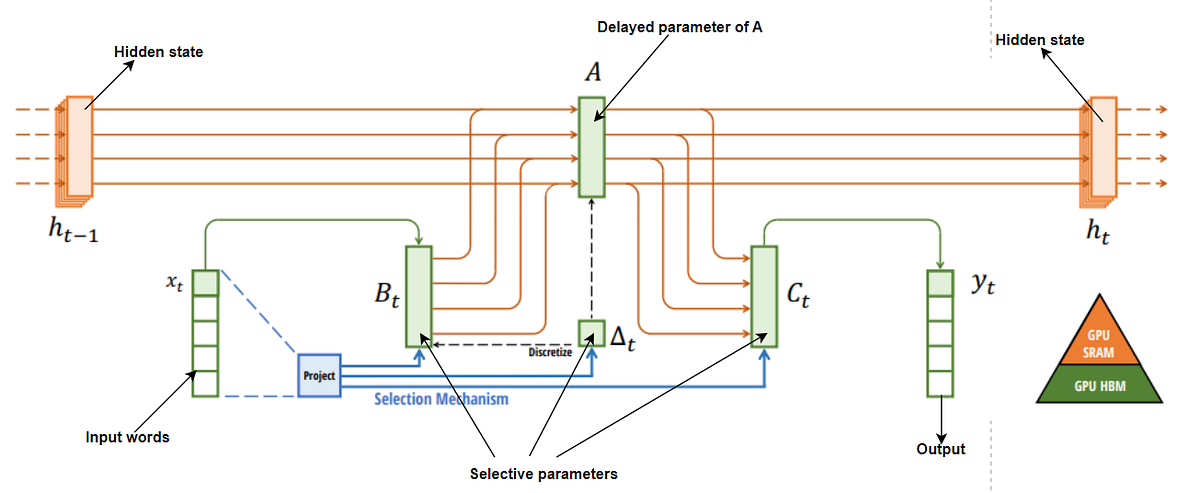
\includegraphics[width=\linewidth]{results/mamba_ssd_s6.png}
    \caption{Mamba: Linear-Time Sequence Modeling with Selective State Spaces. Structured SSMs independently map each channel (e.g. $D$ = 5) of an input $x$ to output $y$ through a higher dimensional latent state $h$ (e.g. $D$ = 4). Prior SSMs avoid materializing this large effective state ($DN$ times batch size $B$ and sequence length $L$) through clever alternate computation paths requiring time-invariance: the ($\Delta$, $A$, $B$, $C$) parameters are constant across time. Our selection mechanism adds back input-dependent dynamics, which also requires a careful hardware-aware algorithm to only materialize the expanded states in more efficient levels of the GPU memory hierarchy}
    \label{fig:mamba_ssd_s6}
\end{figure}

\subsection{Mamba-2: Structured State Space Duality}\label{sec:mamba-2-structured-state-space-duality}

\textbf{Mamba-2 (SSD)} \cite{DaoGu2024TransformersSSM} reformulates the selective state space model through an algebraic duality between linear recurrences and structured matrix multiplications. The key theoretical insight is that the SSM output can be expressed as:

\begin{equation}\protect\phantomsection\label{eq:mamba-ssd-output}{y_i = \sum_{j \leq i} \mathbf{C}_i^\top \left(\prod_{k=j+1}^{i} \bar{\mathbf{A}}_k\right) \mathbf{B}_j u_j
}\end{equation} 
\addcontentsline{equ}{listequations}{\protect\numberline{\theequation}\quad mamba-ssd-output}

Defining the \textbf{SSM matrix} \(M \in \mathbb{R}^{n \times n}\) with entries:

\begin{equation}\protect\phantomsection\label{eq:mamba-ssd-matrix}{M_{ij} = \begin{cases} \mathbf{C}_i^\top \bar{\mathbf{A}}_{j+1:i} \mathbf{B}_j & i \geq j \\ 0 & i < j \end{cases}
}\end{equation} 
\addcontentsline{equ}{listequations}{\protect\numberline{\theequation}\quad mamba-ssd-matrix}

the output is \(\mathbf{y} = M \cdot (\mathbf{B} \odot \mathbf{u})\). The matrix \(M\) is lower-triangular (causal) and \textbf{semi-separable} (each entry factors as an outer product of left and right vectors with a diagonal product in between). This algebraic structure enables efficient chunk-parallel computation:

\begin{enumerate}
\def\labelenumi{\arabic{enumi}.}
\tightlist
\item
  \textbf{Divide} the sequence into chunks of length \(L\).
\item
  \textbf{Within each chunk}, build the \(L \times L\) local SSM matrix and compute the output via a single batched matrix multiply.
\item
  \textbf{Between chunks}, propagate the state once per chunk (rather than once per time step).
\end{enumerate}

The per-chunk cost is \(O(L^2 N)\) for matrix construction and \(O(L^2 d)\) for the matrix-vector product, where \(N\) is the state dimension and \(d\) is the model dimension. With \(n/L\) chunks, the total cost is \(O(n \cdot L \cdot N + n \cdot L \cdot d)\), which for small \(L\) (e.g., \(L = 8\) or \(L = 32\)) is effectively \(O(n)\) with a favorable constant. The critical advantage over $S_6$ is that the intra-chunk computation is \textbf{fully parallel} : a batched matmul rather than a sequential scan : making it much faster on GPUs where parallelism is cheap and sequential operations incur kernel-launch overhead.

The ``\emph{duality}'' in the name refers to the equivalence between the recurrent view (state propagation) and the matrix view (structured matmul): the same computation can be expressed either way, and the implementation can choose whichever is more efficient for the hardware and sequence length. This thesis demonstrates this duality empirically: at \(n = 11\), the recurrent $S_6$ view is faster; at \(n = 255\), the matrix SSD view dominates. 

Mamba-2 can be viewed as a streamlined evolution of Mamba-1: it restructures the block so that the state-space parameters are formed upfront (rather than being generated sequentially along the SSM pathway), and it further stabilizes training by adding an extra normalization stage in the spirit of \emph{NormFormer} \cite{shleifer2021normformer}. In addition, Mamba-2 emphasizes more parallel, consolidated parameter projection (e.g., producing multiple SSM-related tensors via fewer projections) and reduces per-head redundancy by sharing the BBB and CCC projections across heads—conceptually similar to multi-value attention. Figure~\ref{fig:mamba2-ssd-2} presents a comparison of Mamba-SSM and Mamba-2-SSD \cite{dao2024transformersssmsgeneralizedmodels}:

\begin{figure}[H]
    \centering
    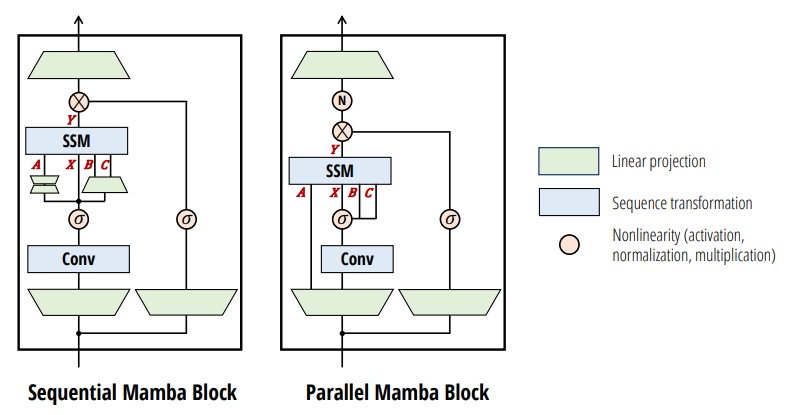
\includegraphics[width=1\linewidth]{results/mamba2_ssd_2.png}
    \caption{ The Mamba-2 block simplifies the Mamba block by removing sequential linear projections; the SSM parameters $A,B,C$ are produced at the beginning of the block instead of as a function of the SSM input $X$ An additional normalization layer is added as in \emph{NormFormer} \cite{shleifer2021normformer}, improving stability. The $B$ and $C$ projections only have a single head shared across the $X$ heads, analogous to multi-value attention (MVA).}
    \label{fig:mamba2-ssd-2}
\end{figure}
\subsection{State Space Models for Signal Processing}\label{sec:state-space-models-for-signal-processing}

The application of state space models to physical-layer signal processing is largely unexplored. Classical signal processing relies extensively on LTI state space models (Kalman filters, Wiener filters), and the SSM framework provides a natural neural extension of these classical tools. The connection is direct: a trained SSM with fixed (input-independent) parameters implements a learnable linear filter, while the selective Mamba variant implements a learnable \emph{adaptive} filter. For the relay denoising task, this means Mamba can potentially learn the optimal filter structure from data, without requiring manual specification of filter order, cutoff frequencies, or adaptation algorithms.

This thesis presents the first comparison of Mamba $S_6$, Mamba-2 (SSD), and Transformers for relay communication, demonstrating that state space models are well suited to this domain and that the SSD formulation of Mamba-2 yields significant speed advantages at longer context lengths.


\section{Theoretical Foundations: Channel Models}\label{sec:theoretical-foundations-channel-models}

This section presents the theoretical BER analysis for each channel model used in this study, derives the closed-form expressions, and validates them against Monte Carlo simulation. The theoretical-simulative comparison serves two purposes: (i) it verifies the correctness of the simulation framework, and (ii) it establishes the baseline performance that AI relays must beat.

\subsection{AWGN Channel : Theoretical Analysis}\label{sec:awgn-channel-theoretical-analysis}

The AWGN channel adds zero-mean Gaussian noise to the transmitted signal: (Equation~\ref{eq:awgn-channel})

\begin{equation}\protect\phantomsection\label{eq:awgn-channel}{y = x + n, \quad n \sim \mathcal{N}(0, \sigma^2), \quad \sigma^2 = \frac{P_s}{\text{SNR}_{\text{linear}}}
}\end{equation} 
\addcontentsline{equ}{listequations}{\protect\numberline{\theequation}\quad awgn-channel}

where \(P_s = \mathbb{E}[|x|^2] = 1\) for unit-power BPSK symbols. The noise variance is inversely proportional to the linear SNR.

\subsubsection{Single-hop BER}\label{sec:awgn-single-hop-ber}
 For BPSK \(\pm 1\) symbols and real-valued AWGN with variance \(\sigma^2 = 1/\text{SNR}\), an error occurs when the noise pushes the received sample past the decision boundary at the origin. The theoretical BER is: (Equation~\ref{eq:awgn-ber})

\begin{equation}\protect\phantomsection\label{eq:awgn-ber}{P_e^{\text{AWGN}} = Q\!\left(\frac{1}{\sigma}\right) = Q\left(\sqrt{\text{SNR}}\right) = \frac{1}{2}\,\text{erfc}\!\left(\sqrt{\frac{\text{SNR}}{2}}\right)
}\end{equation} 
\addcontentsline{equ}{listequations}{\protect\numberline{\theequation}\quad awgn-ber}

where \(Q(x) = \frac{1}{2}\text{erfc}(x/\sqrt{2})\) is the Gaussian Q-function and \(\text{SNR} = P_s / \sigma^2\) is the ratio of signal power to noise variance.

\begin{quote}\label{noise-convension}
\textbf{Noise-convention note.} The standard textbook result \(P_e = Q(\sqrt{2 E_b/N_0})\) assumes that the one-sided noise PSD is \(N_0\), giving a baseband noise variance of \(N_0/2\) per real dimension. In our AWGN implementation the noise is purely real with variance \(\sigma^2 = P_s/\text{SNR}\), so \(N_0 = 2\sigma^2 = 2P_s/\text{SNR}\) and \(E_b/N_0 = \text{SNR}/2\). Substituting yields \(Q(\sqrt{2 \cdot \text{SNR}/2}) = Q(\sqrt{\text{SNR}})\), which is the expression used throughout this work.

By contrast, the fading channels add \textbf{complex} Gaussian noise with total power \(1/\text{SNR}\) (i.e.~\(\sigma_I^2 = \sigma_Q^2 = 1/(2\,\text{SNR})\)) and extract the real part after ZF equalization, halving the effective noise variance per decision dimension. This naturally introduces a factor of 2 inside the Q-function argument for all fading-channel BER expressions (the fading-channel analysis above), making them consistent with the standard textbook forms.
\end{quote}

\subsubsection{Two-hop AF BER}\label{sec:awgn-two-hop-af-ber}
For amplify-and-forward with equal-SNR hops, the effective end-to-end SNR is:

\begin{equation}\protect\phantomsection\label{eq:af-snr-eff}{\text{SNR}_{\text{eff}}^{\text{AF}} = \frac{\text{SNR}_1 \cdot \text{SNR}_2}{\text{SNR}_1 + \text{SNR}_2 + 1} = \frac{\gamma^2}{2\gamma + 1}
}\end{equation} 
\addcontentsline{equ}{listequations}{\protect\numberline{\theequation}\quad af-snr-eff}

where 
\(\gamma = \text{SNR}\) is the per-hop SNR. The resulting BER is

\begin{equation}\protect\phantomsection\label{eq:af-p-eff}{P_e^{\text{AF}} = Q\left(\sqrt{\text{SNR}_{\text{eff}}}\right) 
}\end{equation} 
\addcontentsline{equ}{listequations}{\protect\numberline{\theequation}\quad af-p-eff}

under the same real-noise convention \ref{noise-convension} as the single-hop case.At high SNR, 

\begin{equation}\protect\phantomsection\label{eq:gamma-high-snr}{\text{SNR}_{\text{eff}} \approx \frac{\gamma}{2}}
\end{equation}
\addcontentsline{equ}{listequations}{\protect\numberline{\theequation}\quad gamma-high-snr}


confirming the well-known 3 dB penalty of AF relaying.

\begin{figure}[H]
\centering
\centering
\pandocbounded{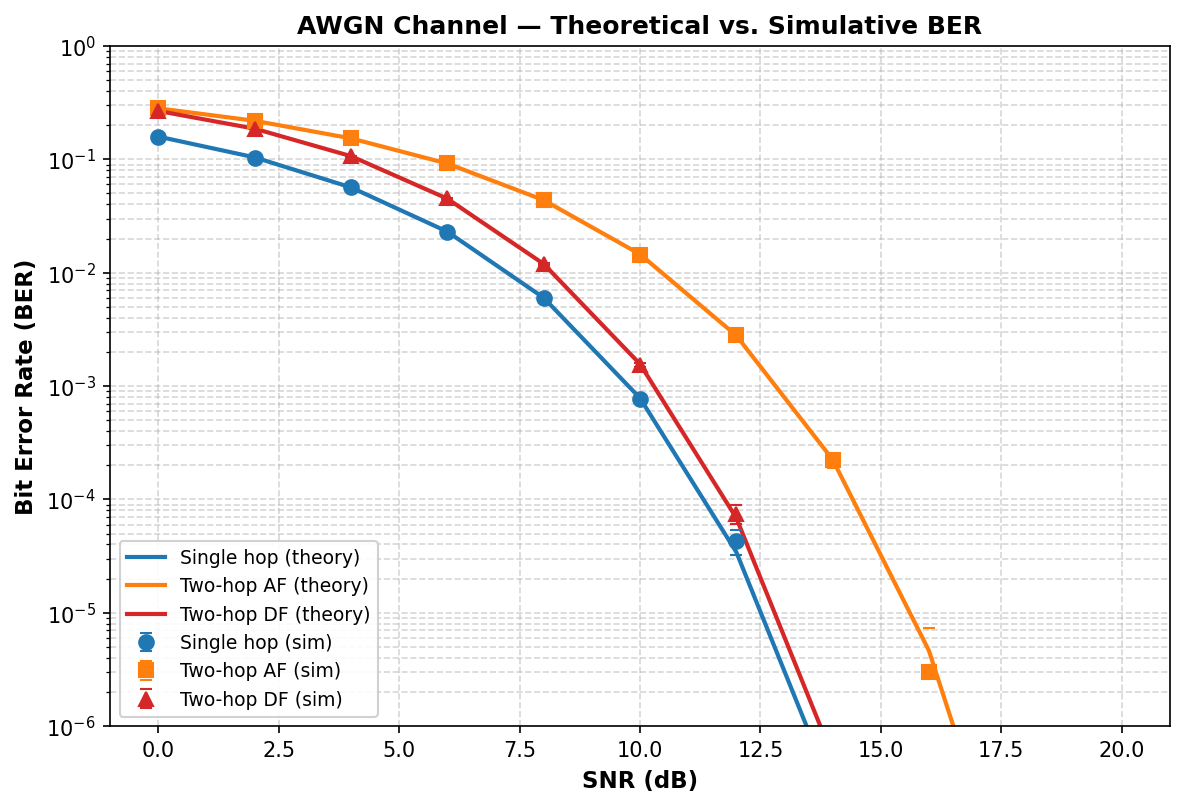
\includegraphics[width=\linewidth,height=0.45\textheight,keepaspectratio]{results/channel_theoretical_awgn.png}}
\caption{AWGN channel : theoretical BER (solid lines) vs.~Monte Carlo simulation (markers with 95\% CI) for single-hop, two-hop AF, and two-hop DF.}\label{fig:fig1}
\end{figure}

\subsubsection{Two-hop DF BER}\label{sec:awgn-two-hop-df-ber}
For a decode-and-forward relay with equal-SNR hops, an error occurs at the destination if exactly one hop introduces an error:

\begin{equation}\protect\phantomsection\label{eq:df-ber-awgn}{P_e^{\text{DF}} = P_{e,1} + P_{e,2} - 2P_{e,1}P_{e,2}
}\end{equation} 
\addcontentsline{equ}{listequations}R{\protect\numberline{\theequation}\quad df-ber-awgn}

With equal hops (i.e. \(P_{e,1} = P_{e,2} = P_e^{\text{AWGN}}\)), this becomes 

\begin{equation}\protect\phantomsection\label{eq:equal-hop-snr}{P_e^{\text{DF}} = 2P_e(1 - P_e)}
\end{equation}\addcontentsline{equ}{listequations}{\protect\numberline{\theequation}\quad equal-hop-snr}

At high SNR, \(P_e \ll 1\) and
\begin{equation}\protect\phantomsection\label{eq:df-high-snr-two-hop-penalty}{P_e^{\text{DF}} \approx 2P_e}
\end{equation}\addcontentsline{equ}{listequations}{\protect\numberline{\theequation}\quad df-high-snr-two-hop-penalty}

, i.e., the two-hop penalty is approximately a factor of 2 in BER.

\subsection{Rayleigh Fading Channel : Theoretical Analysis}\label{sec:rayleigh-fading-channel-theoretical-analysis}

The Rayleigh fading channel models non-line-of-sight (NLOS) propagation where the signal undergoes multiplicative fading:

\begin{equation}\protect\phantomsection\label{eq:rayleigh-channel}{y = hx + n, \quad h \sim \mathcal{CN}(0, 1), \quad n \sim \mathcal{CN}(0, \sigma^2)
}\end{equation} 
\addcontentsline{equ}{listequations}{\protect\numberline{\theequation}\quad rayleigh-channel}

The fading coefficient \(h\) is a circularly-symmetric complex Gaussian random variable, so its magnitude \(|h|\) follows a Rayleigh distribution:

\begin{equation}\protect\phantomsection\label{eq:rayleigh-pdf}{f_{|h|}(r) = 2r \cdot e^{-r^2}, \quad r \geq 0
}\end{equation} 
\addcontentsline{equ}{listequations}{\protect\numberline{\theequation}\quad rayleigh-pdf}

with \(\mathbb{E}[|h|^2] = 1\) (unit average power). The instantaneous SNR after equalization (\(\hat{x} = y/h\)) becomes \(\gamma_h = |h|^2 \cdot \text{SNR}\), which is exponentially distributed.

\subsubsection{Single-hop BER}\label{sec:rayleigh-single-hop-ber}
Averaging the conditional BER \(P_e(\gamma_h) = Q(\sqrt{2\gamma_h})\) over the exponential distribution of \(\gamma_h\) yields the closed-form {[}21, Eq. 14-4-15{]} (Equation~\ref{eq:rayleigh-ber}):

\begin{equation}\protect\phantomsection\label{eq:rayleigh-ber}{P_e^{\text{Rayleigh}} = \frac{1}{2}\left(1 - \sqrt{\frac{\bar{\gamma}}{1 + \bar{\gamma}}}\right)
}\end{equation} 
\addcontentsline{equ}{listequations}{\protect\numberline{\theequation}\quad rayleigh-ber}

where \(\bar{\gamma} = \text{SNR}\) is the average SNR. At high SNR (\(\bar{\gamma} \gg 1\)):

\begin{equation}\protect\phantomsection\label{eq:rayleigh-ber-approx}{P_e^{\text{Rayleigh}} \approx \frac{1}{4\bar{\gamma}}
}\end{equation} 
\addcontentsline{equ}{listequations}{\protect\numberline{\theequation}\quad rayleigh-ber-approx}

This \(1/\text{SNR}\) decay is fundamentally slower than the exponential decay of AWGN (\(Q(\sqrt{\gamma}) \sim e^{-\gamma/2}\)), explaining why Rayleigh fading is significantly more challenging. The channel is \textbf{diversity-limited}: deep fades (where \(|h| \approx 0\)) cause errors regardless of the average SNR. Combating this diversity limitation is the primary motivation for the relay architectures studied in this thesis.

\subsubsection{Two-hop DF BER}\label{sec:rayleigh-two-hop-df-ber}
The two-hop DF relay over Rayleigh fading follows the same composition rule as AWGN:

\begin{equation}\protect\phantomsection\label{eq:df-ber-rayleigh}{P_e^{\text{DF,Rayleigh}} = 2P_e^{\text{Rayleigh}}(1 - P_e^{\text{Rayleigh}})
}\end{equation} 
\addcontentsline{equ}{listequations}{\protect\numberline{\theequation}\quad df-ber-rayleigh}

\begin{figure}[H]
\centering
\centering
\pandocbounded{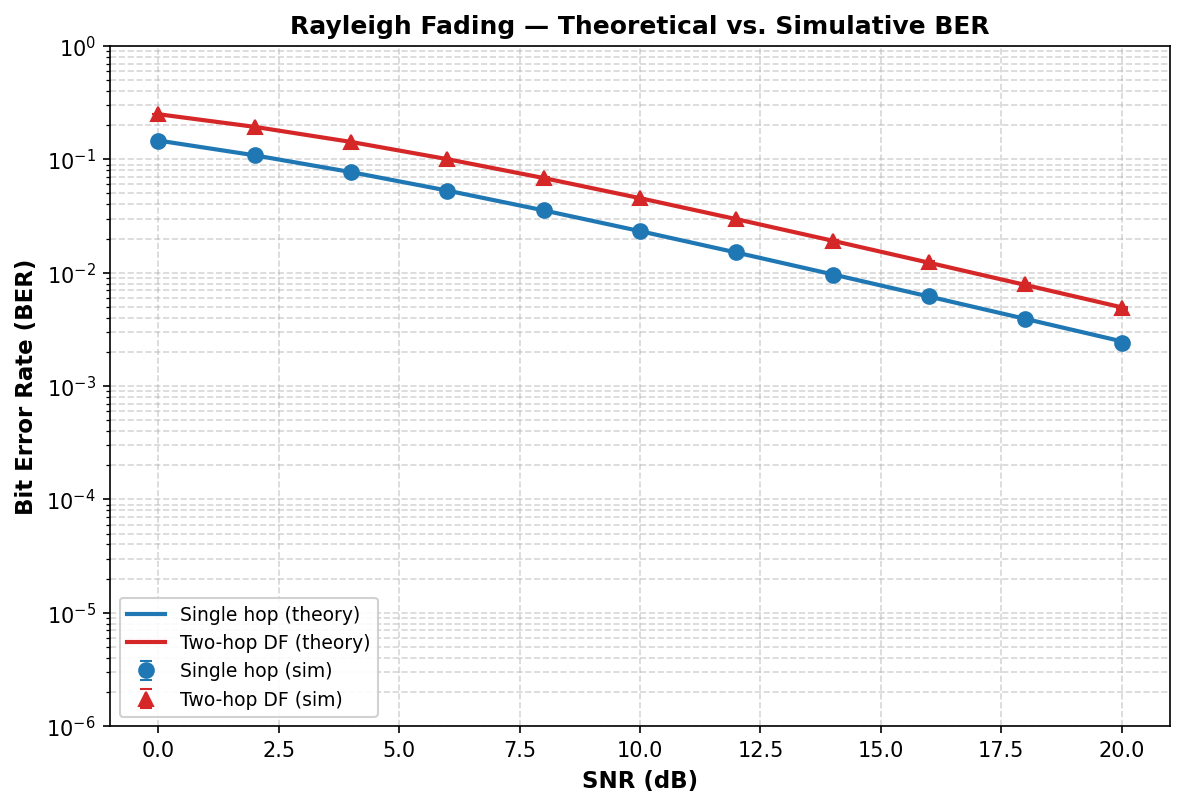
\includegraphics[width=\linewidth,height=0.45\textheight,keepaspectratio]{results/channel_theoretical_rayleigh.png}}
\caption{Rayleigh fading : theory vs.~simulation for single-hop and two-hop DF. The characteristic \(1/\text{SNR}\) slope (compared to the steeper exponential AWGN curve) is clearly visible.}\label{fig:fig2}
\end{figure}

\subsection{Fading Coefficient Distributions}\label{sec:fading-coefficient-distributions}

The statistical behavior of the fading coefficient \(|h|\) determines the severity of fading for each channel model. Figure~\ref{fig:fig4} shows the probability density function (PDF) and cumulative distribution function (CDF) of \(|h|\) for Rayleigh and Rician fading with various K-factors.

\textbf{Key observations from the fading PDFs:}

\begin{itemize}
\tightlist
\item
  \textbf{Rayleigh (\(K=0\)):} The PDF is maximized at \(|h| = 1/\sqrt{2} \approx 0.707\) and has a heavy tail toward zero, meaning deep fades are common. The probability of a deep fade (\(|h| < 0.3\)) is approximately 8.6\%.
\item
  \textbf{Rician \(K=1\):} The LOS component shifts the PDF peak toward higher amplitudes, reducing the probability of deep fades.
\item
  \textbf{Rician \(K=3\):} The distribution becomes more concentrated around the LOS amplitude (\(\nu \approx 0.87\)). Deep fade probability drops to approximately 0.3\%.
\item
  \textbf{Rician \(K=10\):} Approaches a near-deterministic channel; the PDF becomes sharply peaked around \(|h| \approx 0.95\). Fading is negligible.
\end{itemize}

The CDF plot directly shows the \textbf{outage probability} \(P(|h| \leq x)\): for a given threshold \(x\), the CDF value gives the probability that the fading amplitude falls below that threshold. Rayleigh has the highest outage probability at any threshold, confirming its role as the worst-case fading model.

\begin{figure}[H]
\centering
\centering
\pandocbounded{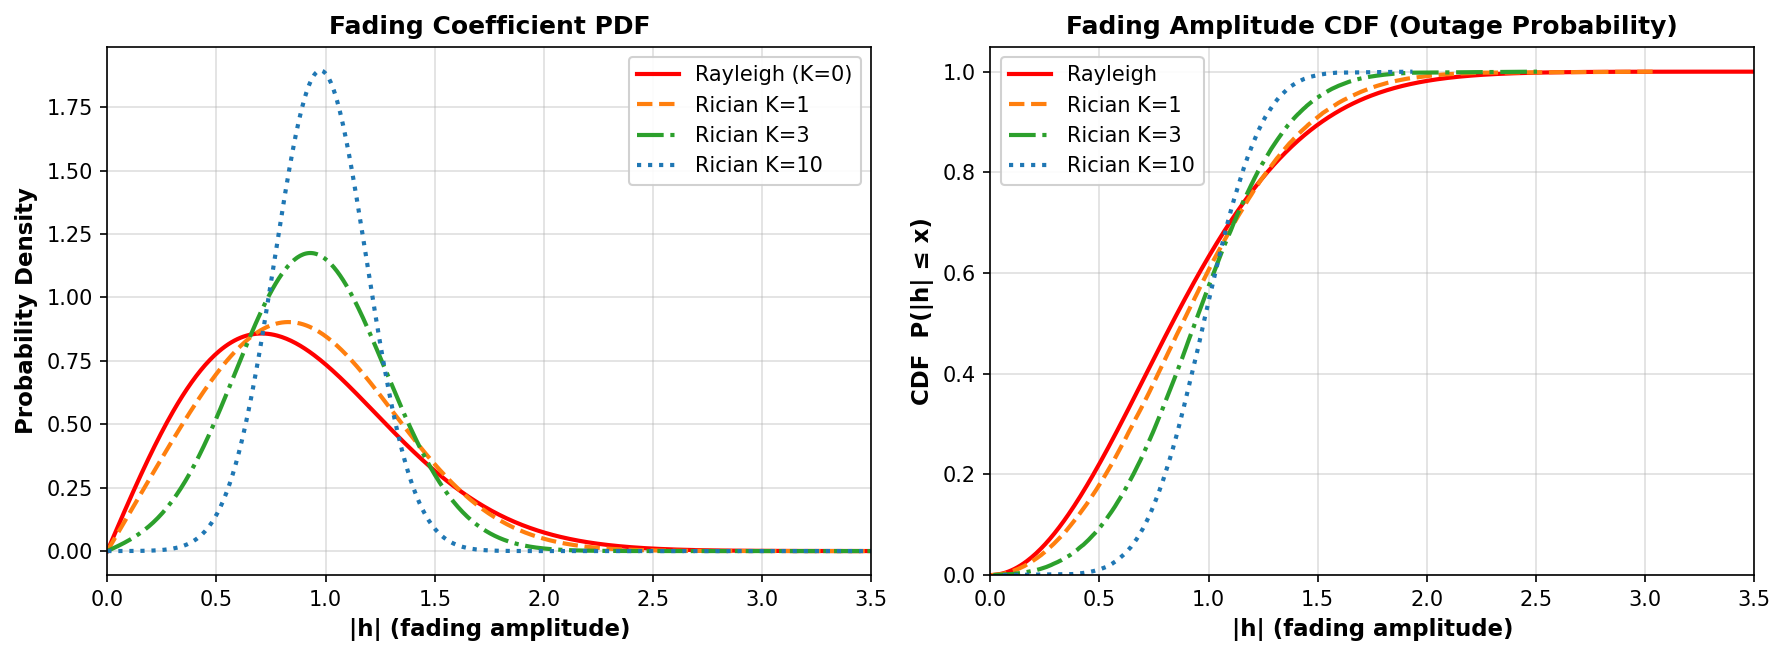
\includegraphics[width=\linewidth,height=0.45\textheight,keepaspectratio]{results/channel_fading_pdf.png}}
\caption{Left : PDF of \(|h|\) for Rayleigh and Rician (\(K=1, 3, 10\)). Right : CDF (outage probability). Rayleigh has the highest deep-fade probability at any threshold.}\label{fig:fig4}
\end{figure}

\subsection{Channel Model Validation (Simulative)}\label{sec:channel-model-validation-simulative}

Before evaluating relay strategies, we validate the simulation framework by comparing Monte Carlo results against the closed-form theoretical BER expressions derived above. For each channel model, 20 independent trials of 50,000 bits per trial are run at each SNR point (0-20 dB, step 2 dB), yielding 1,000,000 total bits per SNR point and tight 95\% confidence intervals.

\textbf{Validation results:}

\begin{itemize}
\tightlist
\item
  \textbf{AWGN:} Simulation matches theory within 95\% CI at all 11 SNR points for single-hop, two-hop AF, and two-hop DF configurations.
\item
  \textbf{Rayleigh:} Simulation confirms the theoretical \(1/(4\bar{\gamma})\) high-SNR slope and matches the closed-form BER within CI bounds.
\end{itemize}



Table A summarizes the theoretical SNR required to achieve a target BER of \(10^{-3}\) on each channel (single-hop BPSK):

\begin{longtable}[]{@{}llll@{}}
\caption{Theoretical SNR required to achieve BER = \(10^{-3}\) on the canonical Rayleigh channel and the AWGN calibration channel (single-hop BPSK).}\label{tbl:table26}\tabularnewline
\toprule\noalign{}
Channel & SNR for BER = \(10^{-3}\) & Diversity Order & High-SNR Slope \\
\midrule\noalign{}
\endfirsthead
\toprule\noalign{}
Channel & SNR for BER = \(10^{-3}\) & Diversity Order & High-SNR Slope \\
\midrule\noalign{}
\endhead
\bottomrule\noalign{}
\endlastfoot
AWGN & \textasciitilde9.8 dB & : (no fading) & Exponential \\
Rayleigh & \textasciitilde24 dB & 1 & \(1/(4\bar{\gamma})\) \\
\end{longtable}

\section{Theoretical Foundations: MIMO Equalization}\label{sec:theoretical-foundations-mimo-equalization}

Three equalization methods were implemented for the 2×2 MIMO topology:

\textbf{Zero-Forcing (ZF):} \begin{equation}\protect\phantomsection\label{eq:zf-equalizer-methods}{\hat{\mathbf{x}}_{\text{ZF}} = (\mathbf{H}^H\mathbf{H})^{-1}\mathbf{H}^H\mathbf{y} = \mathbf{H}^{-1}\mathbf{y}
}\end{equation} 
\addcontentsline{equ}{listequations}{\protect\numberline{\theequation}\quad zf-equalizer-methods}

ZF completely removes inter-stream interference but amplifies noise when \(\mathbf{H}\) is poorly conditioned.

\textbf{MMSE:} \begin{equation}\protect\phantomsection\label{eq:mmse-equalizer-methods}{\hat{\mathbf{x}}_{\text{MMSE}} = (\mathbf{H}^H\mathbf{H} + \sigma^2\mathbf{I})^{-1}\mathbf{H}^H\mathbf{y}
}\end{equation} 
\addcontentsline{equ}{listequations}{\protect\numberline{\theequation}\quad mmse-equalizer-methods}

MMSE adds a noise-variance regularization term that prevents excessive noise amplification, trading residual interference for better noise performance.

\textbf{MMSE-SIC (V-BLAST):}

The SIC equalizer decodes streams sequentially in order of post-detection SINR:

\begin{enumerate}
\def\labelenumi{\arabic{enumi}.}
\tightlist
\item
  \textbf{Ordering:} Compute MMSE post-detection SINR for each stream; select the stream with highest SINR first.
\item
  \textbf{Detection:} Apply MMSE equalization to the selected stream and make a hard decision.
\item
  \textbf{Cancellation:} Subtract the detected stream's contribution: \(\mathbf{y}' = \mathbf{y} - \mathbf{h}_{\text{first}} \hat{x}_{\text{first}}\).
\item
  \textbf{Final Detection:} Estimate the remaining stream interference-free via MRC: \(\hat{x}_{\text{second}} = \text{Re}(\mathbf{h}_{\text{second}}^H \mathbf{y}') / \|\mathbf{h}_{\text{second}}\|^2\).
\end{enumerate}

SIC outperforms linear MMSE because the second stream sees no inter-stream interference after cancellation. The cost is potential error propagation from incorrect first-stream decisions.

All MIMO operations are implemented using vectorized PyTorch batched \texttt{torch.linalg.solve} for GPU acceleration, achieving \textgreater 100× speedup over per-symbol Python loops.

